%
\documentclass[12pt,letterpaper]{article}
\usepackage{bbm}
\usepackage{url}
\usepackage{float}
\usepackage{fancyhdr}
%\usepackage{fancybox}
%\usepackage{amstext}
\usepackage{amsmath}
%\usepackage{rotating}
\usepackage{multicol}
\usepackage{pictexwd}
\usepackage{enumitem}
%\usepackage{booktabs}
\usepackage{graphicx}
\usepackage{booktabs,multirow}
\usepackage{siunitx}
\usepackage{subfigure}
\setlength{\parindent}{0in}
\setlength{\textwidth}{7in}
\setlength{\evensidemargin}{-0.25in}
\setlength{\oddsidemargin}{-0.25in}
\setlength{\parskip}{.5\baselineskip}
\setlength{\topmargin}{-0.5in}
\setlength{\textheight}{9in}
%               Problem and Part
\newcounter{problemnumber}
\newcounter{partnumber}
\newcommand{\Problem}{\stepcounter{problemnumber}\setcounter{partnumber}{0}\item[\makebox{\hfil\textbf{\ \theproblemnumber.}\hfil}]}
\newcommand{\Part}{\stepcounter{partnumber}\item[(\alph{partnumber})]}
\newcommand{\SubPart}{\stepcounter{problemnumber}\setcounter{partnumber}{0}}

\pagestyle{empty}

\rhead{\large\textsc{Angeline Baniqued \& Michael Wee}}
\lhead{\LARGE\textbf{CS 181 Assignment 3}}
\cfoot{}
\renewcommand{\headrulewidth}{0.3pt}
\setlength{\headsep}{40pt}
\usepackage{amssymb}

\begin{document}

\thispagestyle{fancy}\small
  \section*{Problem 1}
        \begin{enumerate}[label={(\alph*)}]
        \item 
For each dimension $i$ of \textit{$\textbf{y}$}, $y_i$ must lie in the range $(x_i - \epsilon, x_i + \epsilon)$ to satisfy max$_m |x_m - y_m| \leq \epsilon$. For each dimension this interval has total length $2\epsilon$. So the probability of this occurring is $(2\epsilon)^M$. 
        \item We have that the pdf of the absolute difference of two standard normal distributions is $2x -x$ for $0 \leq x < 1$. (This was derived as a triangular distribution with parameters ($a=0$, $b=1$, $c=$0)) For the probability $x_i - y_i \leq \epsilon$ in one dimension we have that $\int_0^\epsilon 2 - 2x dx = 2\epsilon - 2\epsilon^2$. In $M$ dimensions, the probability would be $(2\epsilon - 2\epsilon^2)^M$ and since $\epsilon > 0$, we have that $(2\epsilon - 2\epsilon^2)^M \leq(2\epsilon)^M$. 
        \item 
We have that 

\begin{center}

$||\textit{\textbf{x}} - \textit{\textbf{y}}|| = \sqrt{(x_1 - y_1)^2 + \ldots + (x_n - y_n)^2} $ \\[12pt]
$||\textit{\textbf{x}} - \textit{\textbf{y}}||^2 = (x_1 - y_1)^2 + \ldots + (x_n - y_n)^2 \geq$ (max$_{m} |x_m - y_m|)^2$ since the max term is just one of the terms on the left and we are adding strictly positive numbers to it. Taking the square root of both sides, this implies \\[12pt]
$||\textit{\textbf{x}} - \textit{\textbf{y}}|| \geq$ max$_m |x_m - y_m|$ 
\end{center}

We have P(max$_m |x_m - y_m| \leq \epsilon) \leq p$, since we know $||\textit{\textbf{x}} - \textit{\textbf{y}}|| \geq$ max$_m |x_m - y_m|$, the probability of something larger than max$_m|x_m - y_m|$ being less than $\epsilon$ must be even smaller than $p$ since the larger something is, the less likely it is to fit within a certain range. 

        \item We are looking for the lower bound on the number of points needed to guarantee the nearest neighbor of a point \textbf{\textit{x}} will be within a radius $\epsilon$ within it with probability at least $1 - \delta$. We consider the complement, what is required for the nearest neighbor not to be within a radius $\epsilon$. This quantity satisfies $\displaystyle \prod_{i=1}^NP(||\textbf{\textit{x}} - \textbf{\textit{y}}_i|| > \epsilon) \leq (1 - p)^N \leq \delta$. So we have $(1-(2\epsilon)^M)^N \leq \delta$. Solving for $N$, we get $N \geq \displaystyle\frac{\log \delta}{\log(1-(2\epsilon)^M)}$ as a lower bound, where the sign flips because the log quantity is between 0 and 1 and takes a negative value. 

        \item 

This tells us that in high dimensional spaces, points get spread more and more apart. Where $M$ gets larger, we need more and more points as a lower bound to guarantee some probability of having another point within a certain radius of another. This is because as $M$ gets larger, the denominator of the inequality gets smaller, making the overall right hand side of the equation larger. Since points are further and further apart in higher dimensions, it reduces the ability of HAC to correctly group points together into clusters because  as points get further apart, the ability to distinguish clusters based on distances decreases with the metrics we use in HAC.

        \end{enumerate}
  \section*{Problem 2}
        \begin{enumerate}
        \Part
                For the ML method, the predictive distribution is just $P(\boldsymbol{x}|\theta_{MLE})$ where you just compute the maximum likelihood estimate of the parameter
                 $\theta$ given the observed data by taking $argmax_{\theta} P(\mathcal{D}|\theta)$, and then plug it into the distribution function of the new datum. \medskip
                 
                For the MAP method, the predictive distribution is just $P(\boldsymbol{x}|\theta_{MAP})$ where you just compute the maximum a posteriori estimate of the parameter
                 $\theta$ given the observed data by taking $argmax_{\theta} P(\mathcal{D}|\theta)P(\theta)$ and then plug it into the distribution function of the new datum. \medskip
                \medskip
                
                For the FB method, the predictive distribution is just \medskip 
              
                $\displaystyle\int_\theta P(\boldsymbol{x}|\theta)P(\theta|\mathcal{D}) d\theta$ where you just get the posterior distribution $P(\theta|\mathcal{D})$, multiply it by the likelihood,
                
                $P(\boldsymbol{x}|\theta), $ and then integrate it over $\theta$. \medskip
                    
        \Part $MAP$ is more Bayesian because it makes use of the prior distribution on $\theta$ thereby treating $\theta$ as a random variable, 
           unlike $ML$ which assumes that $\theta$\ is fixed.  
        \Part An advantage of MAP over ML is that because one gets to incorporate prior knowledge into the estimation, one gets better parameters when the data is sparse. For example, suppose we want to know the number of occurrences, $X$, of a given word in a document by assuming that $X\sim Bin(N,\theta)$. Suppose we observe very small word counts including many zeros and $\theta$ is quite small. If we use ML, we'll expect the frequency to be zero. However, we most likely suspect that this is not true -- the word may have a very small frequency, but it is still a word and will thus appear occasionally. In the MAP approach, we can account for this by adding a prior on $\theta$ to ensure that the estimate is not 0. \medskip

An advantage of MAP\ over FB is that when the posterior distribution is symmetric and unimodal, it is easier to use the MAP estimate which is just the mode of the posterior distribution, because it is less expensive to compute. The FB\ estimate (the posterior mean) includes integration, thereby increasing computation time.\medskip

 In addition, suppose you have an irregular posterior that is distributed binomially with  $p=0.4$. In this case, 40\%\ of the draws will be 1 and 60\%\ will be 0. The mode (MAP\ estimate) will be 0 and the mean (FB\ estimate) will be 0.4. The MAP\ estimate represents the distribution better than the FB estimate, particularly because the latter value doesn't fall on a value actually obtained in the sample.
        \Part Graphs of $Beta(1,1)$, $Beta(3,3)$, and $Beta(2,5)$ respectively  \medskip
        \begin{figure}[H]
                \centering
                \subfigure[Beta(1,1)]
                {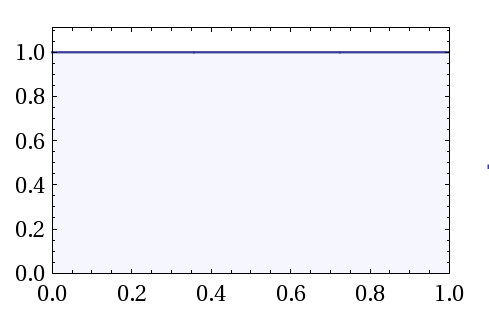
\includegraphics[width=2.3in]{2d_beta11.png}}
                \subfigure[Beta(3,3)]
                {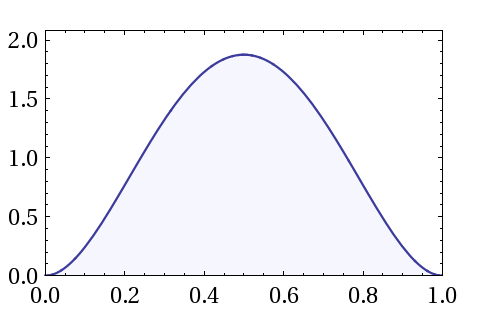
\includegraphics[width=2.3in]{2d_beta33.png}}
                \subfigure[Beta(2,5)]
                {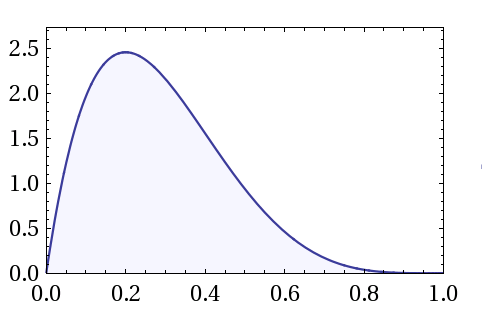
\includegraphics[width=2.3in]{2d_beta25.png}}
        \end{figure}            
        The intuition behind using a $Beta(\alpha, \beta)$ model is to denote the number of wins or losses by the soccer team. We can think of $ \alpha$ as the number of
        successes and $\beta$ as the number of losses. It makes sense to use a $Beta$ distribution as a prior for the probability of a win because the expected value of a $Beta$ 
        distribution is $\alpha/(\alpha+\beta)$ which is just the ratio of past wins to the total number of games the soccer team has played in the past. \medskip

In this case, if we assume a $Beta(1,1)$ prior, that's like saying the team has won once and lost once. The same reasoning holds
         for $Beta(3,3)$ and $Beta(2,5)$. Comparing the shapes of the distributions, $Beta(1,1)$ says the probability of winning is uniformly distributed from $[0,1]$. $Beta(3,3)$ shows 
         that the probability of winning is concentrated near $0.5$. $Beta(2,5)$ shows that the probability of winning is skewed to the right because given a past record of 2-5 wins to losses, the probability of winning
        should be pretty low. 
        \Part The $Beta$ distribution is useful when used with MAP estimation for reasoning with Bernoulli (binary) R.V.s because the $Beta$ distribution is the conjugate prior 
        of a Bernoulli. As a conjugate prior, it is convenient to use because the posterior distribution will be in the same family as the prior distribution.\medskip
        \Part Based on $http://www.gocrimson.com/sports/fball/2011-12/schedule$, the Harvard football team won 9 times and lost once in the 2011-2012 season. Also, they won  the first 3 games of the 2012-2013 season. Given this history, $\mathcal{D} = \{1,1,1\}$.\medskip
        
                \begin{enumerate}[ref=(\roman{*})]
                 \item For the ML estimation, solve for $argmax_{\theta} P(\mathcal{D}|\theta).$   \medskip \\
        
            $P(\mathcal{D}|\theta) = \displaystyle \prod_{i=1}^{N} \theta^{\mathcal{D}_i}(1-\theta)^{1-\mathcal{D}_i}= \theta^{\sum\mathcal{D}_i}  (1-\theta)^{N-\sum\mathcal{D}_i}  $ where $N$ is the number of data in $\mathcal{D}$. \medskip
            
            $ log P(\mathcal{D}|\theta)  = \displaystyle \sum{\boldsymbol{D}_i}log(\theta) +\displaystyle (N-\boldsymbol{\sum D}_i)log(1-\theta)$\medskip
            
            $  \displaystyle\frac{\partial{log(P(\mathcal{D}|\theta))}}{\partial{\theta}} =  \displaystyle \frac{\sum{\boldsymbol{D}_i}}{\theta} -  \frac{N-\sum{\boldsymbol{D}_i}}{1- \theta} = 0$ \medskip 
            
            Solving for $\theta$, we get $\theta_{MLE} = \displaystyle \frac{\sum{\boldsymbol{D}_i}}{N} = 3/3 = 1.  $ Probability of winning the next game is 1. \medskip \\
            
        
                \item For the $MAP$  estimation, we'll use the prior $Beta(9,1)$ and we'll solve \medskip
                
                 $argmax_{\theta} P(\mathcal{D}|\theta)P(\theta).$ \medskip
                
                $P(\mathcal{D}|\theta)P(\theta)=\displaystyle\left(  \prod_{i=1}^{N} \theta^{\mathcal{D}_i}(1-\theta)^{1-\mathcal{D}_i} \right)\frac{\theta^{9-1}(1-\theta)^{1-1}}{\Gamma(9,1)}$ \\
                
               $ \propto \displaystyle\left(  \prod_{i=1}^{N} \theta^{\mathcal{D}_i}(1-\theta)^{1-\mathcal{D}_i} \right)\theta^{8} =  \theta^{\sum\mathcal{D}_i}  (1-\theta)^{N-\sum\mathcal{D}_i}\theta^{8}}  $ \medskip
 
                $\propto   \theta^{8+\sum\mathcal{D}_i}  (1-\theta)^{N-\sum\mathcal{D}_i}$  \medskip
                
                $ log(P(\mathcal{D}|\theta)P(\theta)) =  (8+\sum\mathcal{D}_i)log(\theta) + (N-\sum\mathcal{D}_i)log(1-\theta) $ \medskip
                
                $  \displaystyle\frac{\partial{log(P(\mathcal{D}|\theta)P(\theta))}}{\partial{\theta}} =  \frac{(8+\sum\mathcal{D}_i)}{\theta}-  \frac{(N-\sum\mathcal{D}_i)}{1-\theta} = 0$
                
                Solving for $\theta$, we get $\theta_{MAP} = \displaystyle \frac{8+\sum{\boldsymbol{D}_i}}{N+8} = (8+3)/(3+8) = 1   $ \medskip
                
                Probability of winning the next game is 1.\bigskip
                
                \item  For the $Fully  Bayesian$  estimation, we'll again use the prior $Beta(9,1).$ \medskip
                
                $P(x=1|\mathcal{D}) = \displaystyle \int_{0}^1P(x=1|\theta)P(\theta)d\theta$ \medskip
                   
                 $P(\mathcal{D}|\theta)P(\theta)=\displaystyle\left(  \prod_{i=1}^{N} \theta^{\mathcal{D}_i}(1-\theta)^{1-\mathcal{D}_i} \right)\frac{\theta^{9-1}(1-\theta)^{1-1}}{\Gamma(9,1)}$ \\
                
               $ \propto \displaystyle\left(  \prod_{i=1}^{N} \theta^{\mathcal{D}_i}(1-\theta)^{1-\mathcal{D}_i} \right)\theta^{8} =  \theta^{\sum\mathcal{D}_i}  (1-\theta)^{N-\sum\mathcal{D}_i}\theta^{8}}  $ \medskip
 
                $\propto   \theta^{8+\sum\mathcal{D}_i}  (1-\theta)^{N-\sum\mathcal{D}_i}      $ \\
                
                From here, we can transform this into a $Beta(9+\sum\mathcal{D}_i,N-\sum\mathcal{D}_i+1) $ by multiplying and dividing the expression by a proportionality constant so that when we do the integration, the PDF\ of that beta distribution just becomes 1. The integration basically computes $\mathbb{E}(\theta|\mathcal{D)}$ and since we know that the expected value of $Beta(\alpha,\beta) $ is $\alpha/(\alpha+\beta)$, the probability of winning the next game is just $\displaystyle \frac{(9+\sum\mathcal{D}_i)}{(N-\sum\mathcal{D}_i+1+9+\sum\mathcal{D}_i)}=\frac{9+3}{3+10}\approx 0.92.\ $ \medskip
                \medskip
                
                Probability of winning the next game is 0.92.
                \end{enumerate} 
       \end{enumerate}
  \section*{Problem 3}
  \Problem
        \begin{enumerate}
        \Part We have that the loss function for k-means is as follows: 
\begin{center}
$\displaystyle\sum_n\sum_k r_{nk} ||\textbf{\textit{x}}_n - \textit{\textbf{$\mu$}}_k||^2$  \\
$\displaystyle\sum_n\sum_k r_{nk} (\textbf{\textit{x}}_n - \textit{\textbf{$\mu$}}_k)\cdot (\textbf{\textit{x}}_n - \textit{\textbf{$\mu$}}_k)$ \\
$\displaystyle\sum_n\sum_k r_{nk} [(x_n^1 - \mu_k^1)^2 + (x_n^2 - \mu_k^2)^2 + \ldots + (x_n^n - \mu_k^n)^2]$ \\
\end{center}


We perform gradient descent on this loss function by taking the partial derivative with respect to each entry in the \textbf{\textit{$\mu$}} vector: 
\begin{center}
$\displaystyle\frac{\partial L}{\partial \mu_k} = \sum_n 2 r_{nk} (\textbf{\textit{$\mu$}}_k - \textbf{\textit{x}}_n) = 0$\medskip

Solving for $\mu_k$ we get \medskip

$\displaystyle\sum_n r_{nk} \textbf{\textit{$\mu$}}_k = \sum_n r_{nk} \textbf{\textit{x}}_n$ and \\
$\displaystyle\mu_k = \frac{\sum_n r_{nk} \textbf{\textit{x}}_n}{\sum_n r_{nk}}$ which is exactly the update rule for the $\mu_k$'s.
\end{center}
To derive the update rule for $r_{nk}$ we notice that we have the constraint $\displaystle \sum_k r_{nk} = 1$. To minimize the loss function, you set $r_{nk} = 1$ when for the argument where $||\textbf{\textit{x}}_n - \mu_k||^2$ is minimized. In more compact notation, this is: 
\begin{center}
$r_{nk} = 1$ for $k = $ argmin$_{k'}$ $||\textbf{\textit{x}}_n - \mu_{k'}||^2$, and $r_{nk} = 0 $ otherwise. \end{center}
 
        \Part PCA and k-means can both be used as feature compression techniques. PCA is used as a dimensionality reduction technique to produce a new set of orthonormal features, called principal components, which are the most salient features of the data. Under the squared-loss compression interpretation, PCA tries to make the projections as close as possible to the original data in as few dimensions as possible and minimize the reconstruction error when carrying out the transformation. Meanwhile k-means attempts to assign data to different clusters while updating the centroid of each cluster according to the data that belong to it, all to attempt to minimize its squared loss objective. If we were to replace each datum with its prototype, this would also be a sort of compression of the data set. However, this kind of compression is not of the dimensionality of the data, but rather of summarizing each individual data point by clumping it with the prototype point in the cluster to which it belongs. \\

        K-means requires a parameter in its model, the number of clusters to find, and the choice for this parameter, which may be difficult to make, has a huge effect on the algorithm�s effectiveness. K-means is very effective when a small number of clusters is sufficient to represent the data while it is not very appropriate to use k-means when the number of clusters is large compared to the number of data points. PCA can run on any data set and will have good results on data that can be linearly reduced. PCA works especially well if the data can also be represented well in a small number of dimensions. It would not be appropriate to use PCA on a dataset that cannot be linearly reduced or a dataset that requires a large number of dimensions to represent well. PCA doesn�t do well where there is no linear reduction where the first few components capture enough variance or if there�s low correlation between the different dimensions of the data. \\

        An example of a dataset where PCA might not do well but K-means will is on data drawn from a multivariate spherical, or also a sort of diagonal, Gaussian. PCA does not do well because it needs basically all of the dimensions in the data in order to represent the Gaussian well. A low dimensional PCA representation wouldn�t be a good representation of the data. K-means would do well because it can represent spherical things in low numbers of clusters (e.g. 1 cluster). \\
        
        An example where k-means might not do well but PCA would, is data that form many clusters on a line. While PCA would do well because the data can essentially be captured very well in one dimension, k-means would not because it would require a large k to be able to be effective in clustering the large number of clusters on the line. In this case k-means doesn�t do well because it can�t reduce dimensionality and it can�t cluster well with small k in the original dimensions. PCA does well here because it works well as long as you can project the data linearly in a small number of dimensions. 
        \end{enumerate}
  \section*{Problem 4}
  \Problem
        \begin{enumerate}
        \Part $K$-means clustering algorithm
                \begin{enumerate}
                        \item Several plots of the number of clusters $K$ vs. mean squared error \\
                                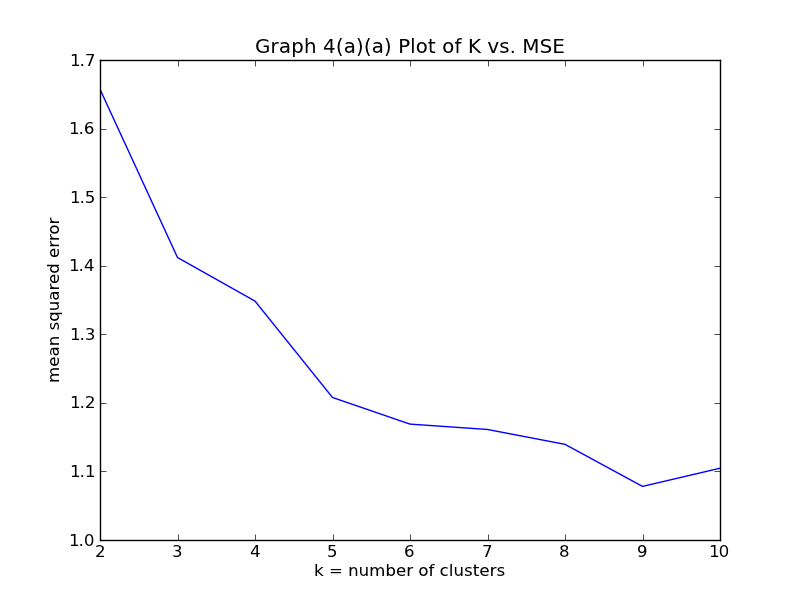
\includegraphics[width=3in]{4aa_fixed_final.png}
                                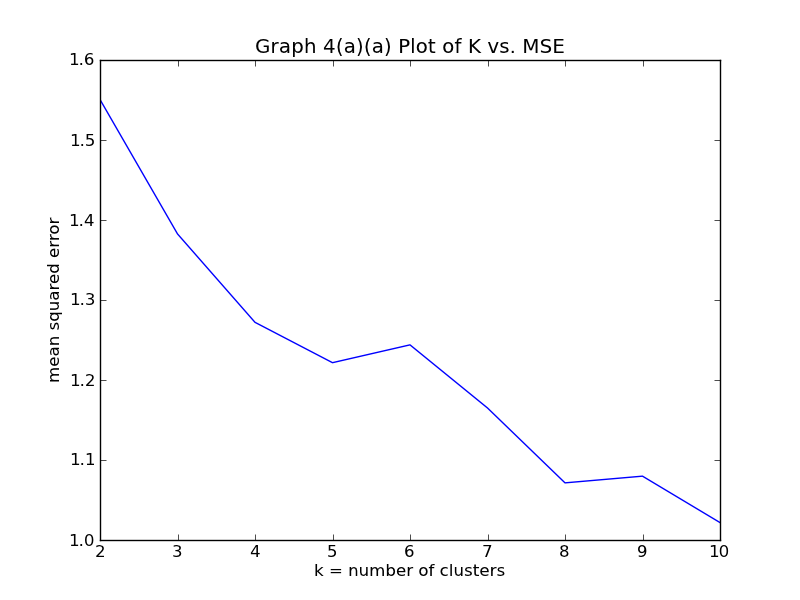
\includegraphics[width=3in]{4aa_fixed_3.png}\\
                        \item Based on the few plots of K versus MSE we generated on different runs of the algorithm, we might choose 5 as the value for K. Looking at the first plot, at K=5, the MSE seems to flatten out such that after K=5, the\ MSE\ doesn't decrease by much. The choice K=5 is supported in the second plot because after K=5, the MSE\ actually increases a little, suggesting that K-means performed a little worse at K=6. Thus, we would choose 5 because it seems to avoid the increase in K=6 and also avoids overfitting effects by choosing a larger value of K.
                \end{enumerate}
        \Part $HAC$ clustering algorithm \medskip
        
        (a) The clusters for max in general cover more data points while in min there are two large clusters and two clusters each containing just one data point. In doing so, max splits a cluster that min recognized as a single cluster into three different clusters. This makes sense as min will only look at minimum distances between clusters, which preclude the two outlier-like points from ever being merged into a cluster since they are so far away. Max does include these two outliers because they lie closer to a large cluster than the large clusters they belong to lie to each other. The clusters in the middle in max reach an equilibrium of how to divide up into 3 different clusters once their maxes are far enough apart. They fit our expectations in that min should produce elongated clusters that create separate clusters for outliers while max produce compact clusters.\\

        Tables and scatter plots comparing clusters formed using min distance metric against clusters formed using the max distance metric: \medskip 
                \begin{enumerate}[label={(\roman*)}]
                        
                        \item For the minimum distance metric: \medskip \\
                        
                        \begin{tabular}{@{}l | c |  c|  c |  c} \hline \hline  \\ [-2ex]
         & $  Cluster 1  $ & $Cluster 2$ &  $Cluster3$ & $Cluster4$ \\ \hline  \noalign{\smallskip}
      Number of instances   & 1     & 1   & 25  &73  \\ \hline \hline

                        \end{tabular}
                        \begin{figure}[H]
                                \centering
                                \caption{Minimum distance metric (x-axis: age, y-axis:\ education, z-axis: income)} {
                                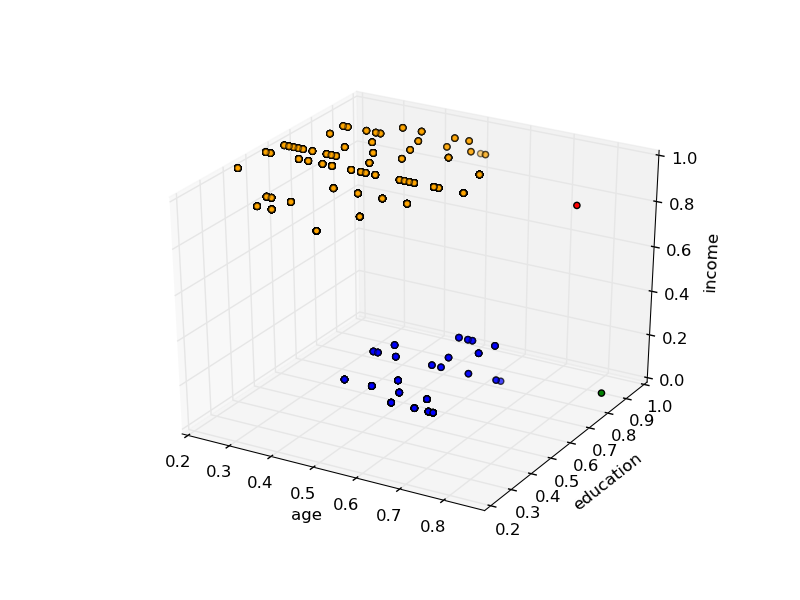
\includegraphics[width=3.5in]{4ba_min.png} }\\
                        \end{figure}
                        \item  For the maximum distance metric: \medskip
                        
                        \begin{tabular}{@{}l | c |  c|  c |  c} \hline \hline  \\ [-2ex]
         & $  Cluster 1  $ & $Cluster 2$ &  $Cluster3$ & $Cluster4$ \\ \hline  \noalign{\smallskip}
      Number of instances   & 19     & 23   & 32  &26  \\ \hline \hline

                        \end{tabular}
                        \begin{figure}[H]
                                \centering
                                \caption{Minimum distance metric (x-axis: age, y-axis:\ education, z-axis: income)} {
                                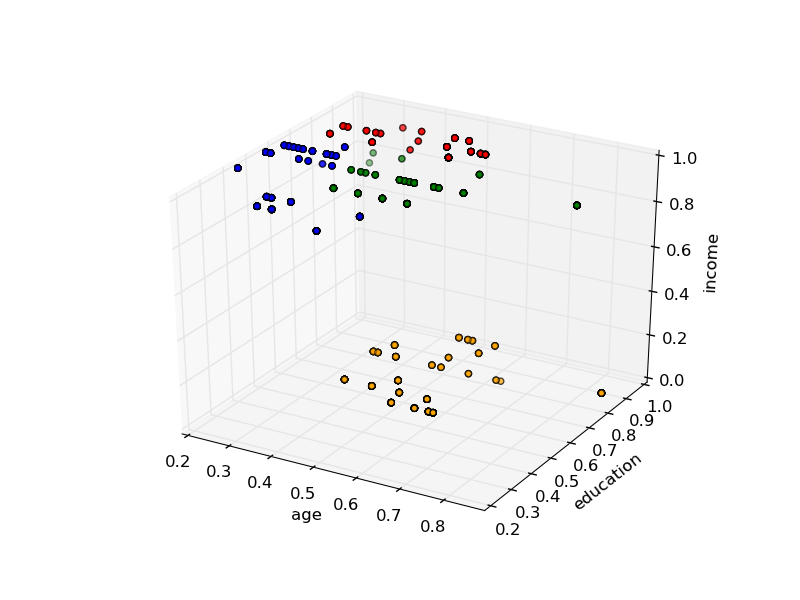
\includegraphics[width=3.5in]{4ba_max.png} }\\
                        \end{figure}
                \end{enumerate}
           (b) The mean and centroid clusters are fairly similar, the only difference being the location of the green cluster: slightly on the left arm of the top cluster in mean, and on the right arm of the top cluster in centroid. This makes sense as both of them are expected to be tradeoffs between compactness and elongation. We would expect them to have similar-looking clusters with small differences since the data given does not have huge variation within clusters and looks like it only has a low number of true clusters.\medskip 

Tables and scatter plots comparing clusters formed using min distance metric against clusters formed using the max distance metric: 
           
            \begin{enumerate}[label={(\roman*)}]
                        
                        \item For the mean distance metric: \medskip \\
                        
                        \begin{tabular}{@{}l | c |  c|  c |  c} \hline \hline  \\ [-2ex]
         & $  Cluster 1  $ & $Cluster 2$ &  $Cluster3$ & $Cluster4$ \\ \hline  \noalign{\smallskip}
      Number of instances   & 1     & 9   & 143  &47  \\ \hline \hline

                        \end{tabular}
                        \begin{figure}[H]
                                \centering
                                \caption{Mean distance metric (x-axis: age, y-axis:\ education, z-axis: income)} {
                                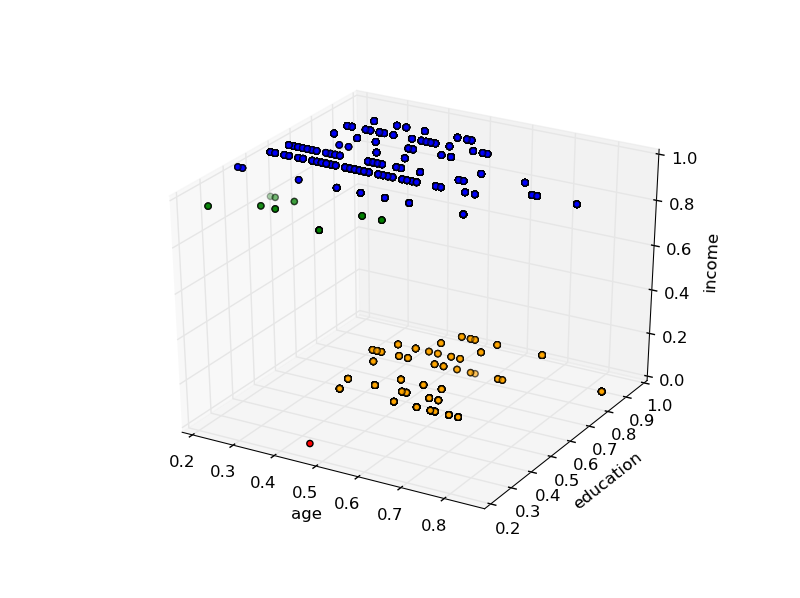
\includegraphics[width=3.5in]{4bb_mean.png} }\\
                        \end{figure}
                        \item  For the centroid distance metric: \medskip
                        
                        \begin{tabular}{@{}l | c |  c|  c |  c} \hline \hline  \\ [-2ex]
         & $  Cluster 1  $ & $Cluster 2$ &  $Cluster3$ & $Cluster4$ \\ \hline  \noalign{\smallskip}
      Number of instances   & 1     & 5   & 147  &47  \\ \hline \hline

                        \end{tabular}
                        \begin{figure}[H]
                                \centering
                                \caption{Centroid distance metric (x-axis: age, y-axis:\ education, z-axis: income)} {
                                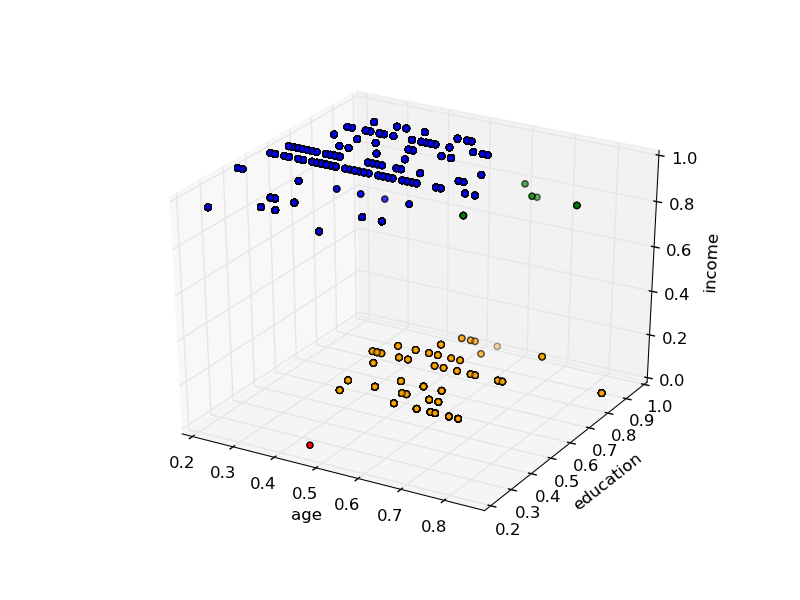
\includegraphics[width=3.5in]{4bb_cent.png} }\\
                        \end{figure}
                \end{enumerate}
        \Part Auto-Class Clustering Algorithm \medskip
        
        In implementing auto-class, we made the continuous attributes discrete by dividing the continuous data into two bins. If the value of that feature/dimension is less than the mean of that feature, then we set it to 0. Otherwise, we set it to 1.                 \begin{enumerate}
                \item By running auto-class with $K=4$ more than once and by using a convergence criterion of \medskip
                

\left| \displaystyle \frac{(log\_likelihood - prev\_log\_likelihood)}{prev\_log\_likelihood}\right| < \epsilon  = 0.00001$,\medskip

 we got several values for the number of iterations before convergence. Because we're starting with random initializations for the parameters, getting inconsistent or several values is not so surprising. By running auto-class 5 times, we got the following number of iterations: 25, 49, 39, 51, and 28.\                  
                \item Although we get different values for the number of iterations before convergence, the log likelihoods that different runs of the algorithm converge to are very close to one another, usually around  $12100 \sim 12300.$ A plot that we got for the auto-class run that produced 28 iterations is below:\\   
                        \includegraphics[width=3in]{auto_class_k4.png}
                  \item The runtime of the K-means clustering algorithm with 4 clusters is around $\sim$ 2 to 3 seconds Examples of specific run times that we got include 2.4, 3.6 and 2.8 seconds. On the other hand, the runtime of the Auto-class clustering algorithm is about $\sim$ 20 to ~70 seconds. Examples of specific run times that we got include 17.0, 51.0 and 70.8 seconds.
As can be seen, the computational complexity of K-means is about $O(n)$ which explains why it ends considerably faster than Auto-class. Auto-class seems to have computational complexity of about $O(n)=nlog(n)$ which explains why the convergence and hence, run times, are slower. 
        \item \textbf{Extra Credit Plots: }\\
                \includegraphics[width=3in]{auto_class_extracredit_2.png}
                \includegraphics[width=3in]{auto_class_extracredit_3.png}\\
                Based on the two different plots of K versus log likelihood that  we generated on different runs of the algorithm, we might choose 5 as the value for K. Looking at the first plot, at K=5, the log likelihood seems to flatten out such that after K=5, the\ log likelihood\ doesn't decrease by much. The choice K=5 is also supported in the second plot because after K=5, the log likelihood\ actually increases a little, suggesting that K-means performed a little worse at K=6. Thus, we would choose 5 because it seems to avoid the increase in K=6 and also avoids overfitting effects by choosing a larger value of K.
                \end{enumerate}
    
                \end{enumerate} 
        \end{enumerate}
  \end{enumerate}
\end{document}
